\documentclass[oneside,10pt]{article}
\usepackage[top=1in, bottom=1in, right=1in, left=1in]{geometry}
\usepackage{amssymb, amsmath, mathrsfs, amsthm}
\usepackage{courier}
\usepackage{graphicx}
\usepackage{color,xcolor}
\usepackage{float}
\usepackage{changepage}
\usepackage{enumitem}
\usepackage{longfigure}
\usepackage{pgfplots}
\usepackage{pgfplotstable}
\usepgfplotslibrary{statistics}
\pgfplotsset{width=10cm,compat=1.9}
\usepackage{tikz}
\usetikzlibrary{tikzmark}
\usepackage{newtxmath}
\usepackage[framemethod=TikZ]{mdframed}
\mdfdefinestyle{MyFrame}{
	linecolor=black,
	outerlinewidth=2pt,
	roundcorner=20pt,
	innertopmargin=\baselineskip,
	innerbottommargin=\baselineskip,
	innerrightmargin=20pt,
	innerleftmargin=20pt,
		}
\title{MATH 5531 Statistical Methods I HW 5}
\author{Russell Land}
\usepackage[color]{statrep}
\def\SRrootdir{/folders/myshortcuts/HW_5}
\def\SRmacropath{/folders/myshortcuts/HW_5/statrep_macros.sas}
\def\SRdefaultdests{latex}

\begin{document}
	\maketitle
		\begin{mdframed} Table 1 shows plasma inorganic phosphate levels (mg/dl) one hour after a standard glucose tolerance test for obese subjects, with or without hyperinsulinemia, and controls (data from Jones, 2017).
			\begin{enumerate}[label=(\alph*)]
				\item Perform a one-factor analysis of variance to test the hypotheses that there are no mean differences among the three groups. What conclusions can you draw?
				\item Obtain a 95\% confidence interval for the differences in means between the two obese groups.
			\end{enumerate}
			\begin{center}
				Table 1: \textit{Plasma Phosphate Levels in Obese and Control Subjects}\\[1mm]
				\renewcommand{\arraystretch}{1.2}
				\begin{tabular}{ c c c}
					\hline
					Hyperinsulinemic Obese & Non-hyperinsulinemic Obese & Control\\
					\hline
					2.3 & 3.0 & 3.0\\
					4.1 & 4.1 & 2.6\\
					4.2 & 3.9 & 3.1\\
					4.6 & 3.3 & 2.1\\
					3.8 & 3.3 & 2.8\\
					5.2 & 3.9 & 3.4\\
					3.1 & & 2.9\\
					3.7 & & 2.6\\
					3.8 & & 3.1\\
					& & 3.2\\
					\hline
				\end{tabular}
			\end{center}
		\begin{enumerate}[label=(\alph*)]
			\addtocounter{enumi}{2}
				\item Apply Fisher's LSD and Tukey multiple comparison procedures to determine where the differences lie (if you reject the null hypothesis).
				\item Using an appropriate model examine the standardized residuals for all the observations to look for any systematic effects and to check the Normality assumptions.
		\end{enumerate} \end{mdframed}
	To answer part (a)--(d) we will be using the SAS Studio Software, University Edition. In this document we will implement a \LaTeX \hspace{0.5mm} package named StatRep. This will allow us to display our SAS code in our \TeX \hspace{0.5mm} document neatly, and will also allow us to compile our SAS results straight into the \LaTeX \hspace{0.5mm} document. Once we present our data below, I will follow up with an analysis of the data. We will begin by creating a data set in the program, and then run the actually procedures for each test. Below shows the data set \texttt{PhosphateLevels} being created:
	\begin{Datastep}[first=8, last=11]
		title 'Inorganic Phosphate Levels';

		data PhosphateLevels;
			input IDNumber Levels;
			datalines;
				1 2.3	
				1 4.1
				1 4.2
				1 4.0
				1 4.6
				1 4.6
				1 3.8
				1 5.2
				1 3.1
				1 3.7
				1 3.8
				2 3.0
				2 4.1
				2 3.9
				2 3.1
				2 3.3
				2 2.9
				2 3.3
				2 3.9
				3 3.0
				3 2.6
				3 3.1
				3 2.2
				3 2.1
				3 2.4
				3 2.8
				3 3.4
				3 2.9
				3 2.6
				3 3.1
				3 3.2
				;
				
				/* IDNumber 1, 2, and 3 correspond to the following:
					1 - Hyperinsulinemic Obese
					2 - Non-hyperinsulinemic Obese
					3 - Control */
					
		run;
	\end{Datastep}
Now that our data set is stored as \texttt{PhosphateLevels}, we can run the appropriate procedures, including \texttt{means},\texttt{anova}, and \texttt{reg}. We will use the \texttt{means} procedure to analyze the means and variance to determine an appropriate test. Since we will be using an \texttt{anova} procedure we have to check if our underlying assumptions hold. That is, we must make sure the samples have a normal distribution, have equal variance, and are independent random samples. Below is the SAS code for our analyses:
	\begin{Sascode}[store=hw]
		proc means;
			by IDNumber;
			
		proc anova;
			class IDNumber;
			model Levels = IDNumber;
			means IDNumber/ lsd tukey;
			
		proc reg;
			id IDNumber;
			model Levels=IDNumber/ cli;
			
		proc print;
		run;
	\end{Sascode}
	
	\Listing[store=hw,
		caption={Statistics for ANOVA, LSD, Tukey, and Residual Analysis}]{tsta}
   
	\Graphic[store=hw,
		scale=0.8,
		caption={Comparative Box Plots for Normality}]{tstb}
\newpage
	\begin{enumerate}[label=(\alph*)]
		\item We are trying to test the hypothesis that there are no mean differences among the three groups, Hyperinsulinemic Obese, Non-hyperinsulinemic Obese, and Control. We can define our hypotheses:
			\begin{adjustwidth}{2.5em}{0pt}
				$H_0: \mu_1 = \mu_2 =\mu_3$\\
				\hspace*{1mm} vs.\\
				$H_A:$ At least one of the three sample means is different from the rest
			\end{adjustwidth}
			From our SAS results, we can see that the \texttt{anova} procedure ran the test for us and returned a final $p$-value of 0.0002. Hence, we have significant evidence to reject the null hypothesis. Thus, there is significant evidence that at least one of the sample means differs from the rest.
		\item For our model it is best to use Tukey's simultaneous confidence intervals. Since we have different sample sizes we had to adjust our value of $W$ to: $$W^{*}=\frac{q_{\alpha}(t,v)}{\sqrt{2}}\sqrt{s_w^2\left(\frac{1}{n_i}+\frac{1}{n_j}\right)}$$ However, using the SAS software we did not have to do any computations ourselves. We obtain a 95\% confidence interval for the difference in means between the two obese groups to be $(-0.1576,1.1735)$. Again, this was computed using the adjusted $W$ value and the formula for the simultaneous confidence interval: $$\left(\bar{y}_i-\bar{y}_j\right)\pm W^{*}$$
		\item From the data we obtained from running the \texttt{lsd} and \texttt{tukey} under the \texttt{means} options we were able to conclude the following results:
		\begin{center}
			\begin{tabular}{ c c c }
				\multicolumn{3}{c}{Fisher's Confidence Intervals}\\
				\hline
				Difference in Means & 95\% C.I. for Difference & Conclusion\\
				\hline
				$\mu_2-\mu_1$ & (-1.0589,0.0430) & Not Significant\\
				$\mu_3-\mu_1$ & (-1.6571,-0.6672) & Significant\\
				$\mu_3-\mu_2$ & (-1.1954,-0.1129) & Significant\\
				\hline
			\end{tabular}
		\end{center}
		\vspace*{4mm}
		\begin{center}
			\begin{tabular}{ c c c }
				\multicolumn{3}{c}{Tukey Confidence Intervals}\\
				\hline
				Difference in Means & 95\% C.I. for Difference & Conclusion\\
				\hline
				$\mu_2-\mu_1$ & (-1.1735,0.1576) & Not Significant\\
				$\mu_3-\mu_1$ & (-1.7600,-0.5642) & Significant\\
				$\mu_3-\mu_2$ & (-1.3079,-0.0004) & Significant\\
				\hline
			\end{tabular}
		\end{center}
		From these results we can see that between both the \texttt{lsd} and \texttt{tukey} results the difference between $\mu_2$ and $\mu_1$ are not significant enough to reject the null, because 0 is contained in the intervals. However, pairwise with the rest of the results, the data is significant enough to reject the null because 0 is not contained in the intervals of the other mean differences. Thus, we can conclude that when using Fisher's LSD and Tukey's LSD test, the majority of difference lies when means are pairwise with the control group, or $\mu_3$. This leads us to believe that $\mu_3$ may have a significant difference from the rest.
		\item To check our normality assumptions we can always analyze the box-plots that were printed when we ran our \texttt{anova} test. However, we can also check using the standardized residuals. These can be computed with the following formula: $$e_{ij}=y_{ij}-\bar{y}_i$$ After applying this formula we obtain the following results for our data set:
	\begin{adjustwidth}{-2cm}{0pt}
		\begin{minipage}{0.45\linewidth}
			\begin{tabular}{ c c c }
				\multicolumn{3}{c}{Residuals for Phosphate Levels}\\
				\hline
				Hyperinsulinemic Obese & Non-hyperinsulinemic Obese & Control\\
				\hline
				-1.6455 & -0.4375 & 0.2167\\
				0.1545 & 0.6625 & -0.1833\\
				0.2545 & 0.4625 & 0.3167\\
				0.0545 & -0.3375 & -0.5833\\
				0.6545 & -0.1375 & -0.6833\\
				0.6545 & -0.5375 & -0.3833\\
				-0.1455 & -0.1375 & 0.0167\\
				1.2545 & 0.4625 & 0.6167\\
				-0.8455 & & 0.1167\\
				-0.2455 & & -0.1833\\
				-0.1455 & & 0.3167\\
				& & 0.4167\\
				\hline
			\end{tabular}
		\end{minipage}
		\hspace*{4cm}
		\begin{minipage}{0.45\linewidth}
		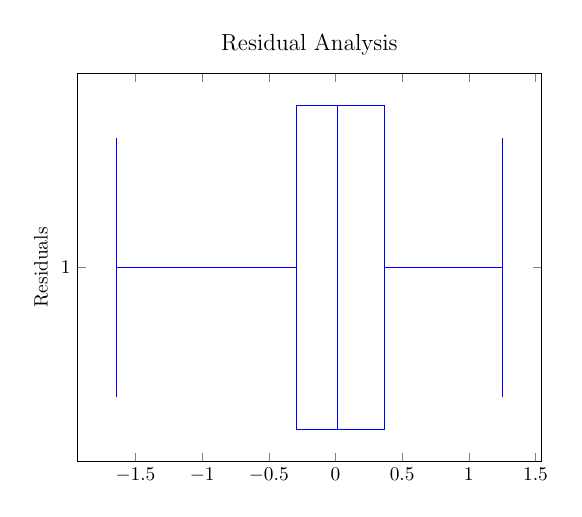
\begin{tikzpicture}[scale=0.7]
					\begin{axis}	[
						title={\large Residual Analysis},
						ytick={1},
						ylabel={Residuals}
							]
				\addplot+[
					boxplot prepared={
						median=0.0166667,
						upper quartile=0.3666667,
						lower quartile=-0.2914773,
						upper whisker=1.2545455,
						lower whisker=-1.6454545
							},
						] coordinates {};
				\end{axis}
			\end{tikzpicture}
		\end{minipage}
		\end{adjustwidth} \vspace*{6mm}
		From the resulting table and graph we can conclude that our data is approximately normal. The median is just about the mean and the box-plot has a considerable symmetric shape. Thus, our normality assumptions were correct for the procedures we ran. Furthermore, along with the other SAS procedures we ran, we can add in the \texttt{proc reg} procedure with the \texttt{cli} option. This will give us similar results as above, but will support our argument more. The corresponding tables and graph will be shown with the rest of the SAS results above.
	\end{enumerate}
\end{document}